\documentclass[a4paper,10pt]{article}

\usepackage{multicol}
\usepackage{caption}
\usepackage[utf8]{inputenc}
\usepackage{hyperref}
\usepackage[left=2cm,right=2cm,bottom=2.5cm]{geometry}
\usepackage{authblk}
\usepackage{graphicx}
\usepackage{subfigure}
\usepackage{amsmath}


\usepackage{tikz}
\usetikzlibrary{calc}

\tikzset{egrid/.style={draw,help lines}}
\tikzset{mgrid/.style={draw,help lines,dashed}}
\tikzset{epoint/.style={draw,circle,red,inner sep=2pt,fill}}
\tikzset{mpoint/.style={draw,circle,blue,inner sep=2pt,fill}}

\graphicspath{{./Slike/}}

\title{Modelling light propagation through \\ optically non-uniform anisotropic materials}
\author[1]{Miha \v Can\v cula\thanks{miha.cancula@student.fmf.uni-lj.si}}
\author[1,2]{Miha Ravnik}
\author[1,2,3]{Slobodan \v Zumer}
\affil[1]{Faculty of Mathematics and Physics, University of Ljubljana, Slovenia}
\affil[2]{Centre of excellence NAMASTE, Ljubljana, Slovenia}
\affil[3]{Jo\v zef Stefan Institute, Ljubljana, Slovenia}

\renewcommand\Authands{ and }


\newcommand{\odvod}[2]{\frac{\partial #1}{\partial #2}}
\renewcommand{\vec}{\mathbf}
\newcommand{\eps}{\varepsilon}
\newcommand{\E}{\vec E}
\newcommand{\B}{\vec B}
\newcommand{\angl}[1]{(\textit{angl. #1})}

\renewenvironment{figure}
  {\par\medskip\noindent\minipage{\linewidth}}
  {\endminipage\par\medskip}
  
\begin{document}
\maketitle
\begin{abstract}
      Liquid crystals are central to modern optics and photonics due to their birefringence and the possibility of external control. 
We present a method for modelling the propagation of light through non-uniform and optically anisotropic materials. 
It is based on the finite-difference time-domain (\textsc{FDTD}) method which evolves electromagnetic fields according to Maxwell's equations. 
Unlike other methods for modelling the flow of light, such as Jones' matrices or the Berreman method, it can describe arbitrarily complex structures which occur in liquid crystals. 
With the newly-implemented method, we calculated the transmittance of a liquid crystal layer between crossed polarizers, which agrees with observations and theoretical predictions. 
The method correctly predicted the position of photonic band gap in 1D photonic crystals. 
Additionally, more optically complex liquid crystalline structures can be considered.
\end{abstract}

\begin{multicols}{2}

\section{Introduction}

Combined birefringence and possibility of external control make liquid crystals uniquely useful for advanced optics and photonics\cite{optics-lcd}. 
Their optical anisotropy is tied to the orientational order, which can be manipulated using confinement, electric or magnetic fields\cite{ravnik-zumer-ldg}. 
Unlike in conventional solid-state birefringent crystals, the birefringence $\Delta n$ and the optical axis in liquid crystals can be spatially varied and manupilated in time. 
Optical properties of liquid crystal are widely used in displays, waveguides, microresonators, and optical switches\cite{coles-morris,humar-musevic}. 
Passing of light through a defect in the orientational order can produce an optical phase singularity, allowing for optical information processing and contactless manipulation of matter\cite{brasselet-droplet}. 

At a classical yet wavelength level, light is described as an electromagnetic field. 
There are several methods of modelling light propagation using a simplified description of light. 
The Jones method treats light as a combination of two transversal components of the electric field and proves practical only for materials with high symmetry\cite{berreman}. 
The Berreman method, with treats transversal components of both electric and magnetic fields, is more commonly used for liquid crystals;
however, it is not suitable for areas with high lateral variations of dielectric tensor, such as around liquid crystal defects\cite{hwang-rey}. 

Here, in order to model the propagation of light through liquid crystals, we go beyond these approxiamtions, and model light as a full electromagnetic field. All six components of electromagnetic fields are considered. 
This is done using the finite-difference time-domain (\textsc{FDTD}) method\cite{taflove,hwang-rey}. 
Note that this method requires large computational resources and is only feasible in recent years due to progress in computer technology. 
In this contribution we present the recent development and application of the FDTD method in several chosen setups, 
including refraction on an interface, a uniform-director liquid crystal cell, and a 1D photonic crystal. 

\section{Methods}
In the finite-difference time-domain method, the electric and magnetic fields are spatially discretized onto a lattice. 
They are then time-evolved according to Maxwell's equations\cite{taflove}. 
In a studied liquid crystal cell, there are no free charges and no currents. 
Using dimensionless units ($c=\varepsilon_0=\mu_0=1$), two of the equations can be written as
\begin{align}
\label{eq:maxwell}
 \odvod{\vec{B}}{t} = -\nabla \times \vec{E}, \qquad \odvod{\vec{E}}{t} = \eps^{-1} (\nabla \times \vec{B})
\end{align}
and the other two equations hold automatically\cite{taflove}. 
It is therefore sufficient to only consider the above two equations. 

\subsection{Lattice}
Using the structure of the two equations and a suitable discretization lattice, the precision of the method can be improved without sacrificing performance. 
Most implementations of the \textsc{FDTD} method use the Yee lattice\cite{yee, taflove, yee-lattice}, shown on Figure \ref{fig:lattice}. 

\begin{figure}
 \centering
 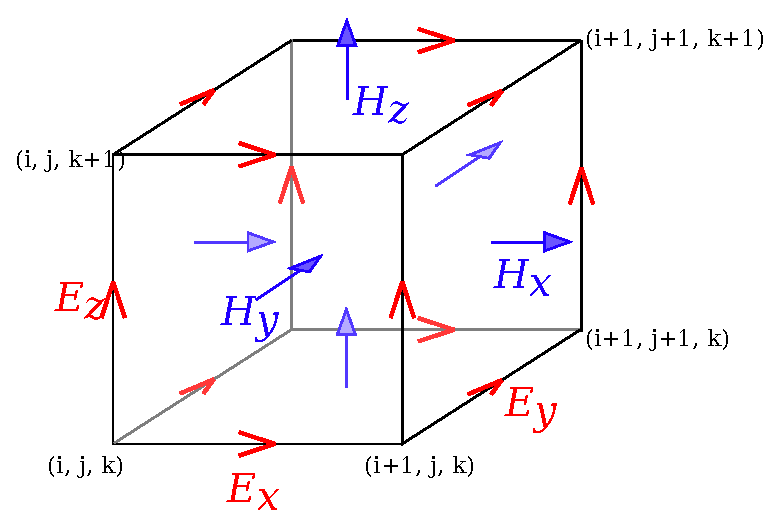
\includegraphics[width=.5\textwidth]{Yee-cube}
 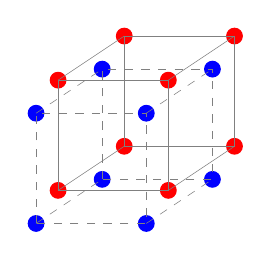
\begin{tikzpicture}[scale=.7]
    
    \foreach \x in {0,1}{
      \foreach \y in {0,1}{
        \node[mpoint] at (2*\x,2*\y) {}; 
        \node[mpoint] at (2*\x+1.2,2*\y+0.8) {}; 
        \node[epoint] at (2*\x+1.6,2*\y+1.4) {};
        \node[epoint] at (2*\x+1.6-1.2,2*\y+1.4-0.8) {};
        \draw[mgrid] (2*\x,2*\y) -- (2*\x+1.2,2*\y+0.8);
        \draw[egrid] (2*\x+1.6,2*\y+1.4) -- (2*\x+1.6-1.2,2*\y+1.4-0.8);
      }
    }
    
    \draw[mgrid] (0,0) rectangle (2,2);
    \draw[mgrid] (1.2,0.8) rectangle (3.2,2.8);
    \draw[egrid] (1.6,1.4) rectangle (3.6,3.4);
    \draw[egrid] (1.6-1.2,1.4-0.8) rectangle (3.6-1.2,3.4-0.8);

            \end{tikzpicture}
 \captionof{figure}{Left: the Yee lattice, where each component of the EM fields is defined at a different site\cite{yee-lattice}. Right: the lattice we used, where all three components of each field are known at the same site. In both cases, electric and magnetic fields are known at different times. }
\label{fig:lattice}
\end{figure}

Using the Yee lattice, the space-derivatives in eq. (\ref{eq:maxwell}) are defined exactly where they are needed for calculating the corresponding time-derivative. 
However, this benefit is only used when the dielectric tensor is diagonal. 
In a liquid crystal with spatially-dependent optical axis, this is not true, so we used a modified lattice to account for a fully-anisotropic dielectric tensor. 

\subsection{Boundary conditions}

Equations (\ref{eq:maxwell}) assume no sources inside the cell. 
This is consistent with experimental setups, where light is transmitted thorugh the sample and then studied. 
In the numerical method, an external light source is modelled using boundary conditions. 

At other walls of the studied cell, we simulate propagation into free space using an absorbing boundary condition. 
The absorbing boundary used is the perfectly matched layer (\textsc{PML}), a non-physicial material where each component of electromagnetic fields is split into two parts. 
Each of these components observes different electric and magnetic conductivity. 

\section{Results}

\subsection{Refraction and reflection}

When a light wave hits an interface between areas with different refractive indexes, a part of the wave is reflected and the rest is refracted. 
The intensity of reflected light depends on the ratio of refractive indexes, the angle of incidence and the polarization of incident light. 
At a certain angle, none of the light with polarization in the plane of the propagation direction and interface normal is reflected. 
This is called Brewster's angle and is equal to
\begin{align}
 \theta_B &= \arctan\left(\frac{n_1}{n_2}\right)\,.
\end{align}
Near this angle, we observe a very weak reflection, while most of the light is refracted according to Snell's law. 
A snapshot of a plane wave hitting an interface near Brewster's angle is presented on Figure \ref{fig:refraction-test}. 

\begin{figure}
 \centering
 \includegraphics[width=\textwidth]{refraction_t}
 \captionof{figure}{Reflection and refraction on an interface near Brewster's angle. Colors show local electric field, while arrows show the direction of propagation of light. }
 \label{fig:refraction-test}
\end{figure}

Four distinct regions are visible on the figure. 
The red region on the left is the absorbing boundary. 
Next to it is the region with incident and reflected light. 
We can cleary see the interface near the middle of the figure. 
On the right side of the interface is the region with a higher index of refraction and correspondingly shorter wavelength. 
The light has not yet reached the rightmost boundary of the cell, so we see another empty region there. 

\subsection{Uniform layer}

A common method for observing liquid crystal and other anisotropic materials is to put a sample between crossed polarizers. 
If the sample is isotropic, no light passes through. 
However, if the material is optically anisotropic, the intensity of transmitted light depends on the orientation of the optical axis, light wavelength $\lambda_0$ and cell thickness $d$. 
If the optical axis is uniform, forming an angle $\theta$ with the transversal plane and $\beta$ with the first polarizer, it is equal to\cite{kleman}
\begin{align}
 I &= I_0 \sin^2 2\beta \sin^2 \left[ \frac{\pi d}{\lambda_0} \left( \frac{n_o n_e}{\sqrt{n_e^2 \cos^2 \theta + n_0^2 \sin^2 \theta}} - n_o \right)\right] \nonumber
\end{align}
where $n_o$ and $n_e$ are the ordinary and extraordinary refractive indices and $I_0$ is the incident light intensity. 

The results of the simulation, compared with the theoretical prediction, are shown on Figure \ref{fig:test-uniform}. 
We can see full agreement, confirming the performance of the method when using an anisotropic material. 

\begin{figure}
\centering
 \resizebox{\textwidth}{!}{\input{g_test_uniform_en}}
 \captionof{figure}{Transmittance of a sample with a uniform and anisotropic dielectric tensor between crossed polarizers}
 \label{fig:test-uniform}
\end{figure}

The setup of two crossed polarizers has a four-fold symmetry axis and four mirror planes. 
The results shown above reproduce this symmetry. 

\subsection{1D photonic crystals}

With a periodic modulation of refractive index, we observe that light of distinct frequencies cannot propagate through the medium\cite{hecht-nano,joannopoulos}. 
This phenomenon is called the photonic bang gap and is related to the electron band gap in semiconductors. 

We used a simple periodic structure -- a 1D photonic crystal made from a stack of different dielectric layers -- as shown on Figure \ref{fig:periodic-structure}. 
We repeated the simulation with various values of both refractive indexes. 

\begin{figure}
 \centering
  \resizebox{\textwidth}{!}{\input{./Slike/periodic-structure.pdf_tex}}
  \captionof{figure}{A periodic structure with alternating layers of different refractive indexes\cite{joannopoulos}}
  \label{fig:periodic-structure}
\end{figure}

A plane wave was sent through the structure in the $z$ direction. 
A theoretical treatment of such a structure predict the relation between light frequency and wave vector as shown on Figure \ref{fig:bandgap}. 

When both dielectric constants are not equal, we find an interval of frequencies where no wave vector is possible. 
Light with such frequencies cannot propagate through the medium and is thus totally reflected. 

\begin{figure}
 \centering
 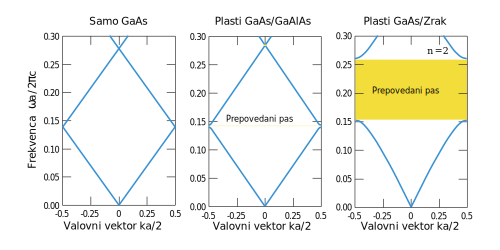
\includegraphics[width=\textwidth]{bandgap}
  \captionof{figure}{Relations between light frequency and wave vector for alternating layers with different refractive indexes\cite{joannopoulos}. The dielectric constant of one layer is 13, while the other is 13 (left), 12 (center) and 1 (right). Yellow regions are photonic band gaps.}
  \label{fig:bandgap}
\end{figure}

Using our numerical method, we sent a plane wave through the same structure and measure the intensity of light at the far end. 
We used light of several different frequencies and expected to find very low intensity when the frequency is in the band gap. 
The results are shown in Figure \ref{fig:test-periodic}. 

\begin{figure}
 \centering
  \resizebox{\textwidth}{!}{\input{g_test_periodic_en}}
  \captionof{figure}{Transmittance of periodic structures depending on their dielectric constants and the frequency of light. Regions with very low transimitivity correspond to the band gap. }
  \label{fig:test-periodic}
\end{figure}

The lower boundary of the band gap is in all cases at normalized frequency $\frac{\omega a}{2\pi}$ just below $0.15$, while the upper boundary depends more strongly on the difference in dielectric constants. 
This result shows strong agreement with the theoretical prediction on Figure \ref{fig:bandgap}. 
The numerical method used gives correct results for the propagation of light through periodic structures. 

\section{Conclusions}
We have implemented a method for modelling the propagation of light through non-uniform and optically anisotropic media, such as liquid crystals. 
This method has proved to correctly predict the phenomena of reflection and refraction on an interface, as well as photonic band gap in periodic structures, both qualitatively and quantitatively.  
When applied to a layer of liquid crystal between crossed polarizers, its results closely matches the theoretical prediction. 

The \textsc{FDTD} method works with arbitrary profiles of dielectric tensor. 
In the light of this results we believe this method could be used to model various complicated profiles of the dielectric tensor. 
We expect the most applications in liquid crystals, where the dielectric tensor is both non-uniform and fully anisotropic. 

\bibliographystyle{zumer}
\bibliography{magisterij}

\end{multicols}

\end{document}
